%%%%%%%%%%%%%%%%%%%%%%%%%%%%%%%%%%%%%%%%%%%%%%
%                insertmeeting
% 1) Title (something creative & funny?)
% 2) Date (MM/DD/YYYY)
% 3) Location (ex. Hagerty High School)
% 4) People/Committees Present 
% 5) Picture 
% 6) Start Time & Stop Time (ex. 12:30AM to 4:30PM)
%%%%%%%%%%%%%%%%%%%%%%%%%%%%%%%%%%%%%%%%%%%%%%
\insertmeeting 
	{ARMageddon Part 2} 
	{02/24/22} 
	{Hagerty High School}
	{James, Jensen, Nathan, Ritam}
	{Images/RobotPics/robot.jpg}
	{2:30 - 6:30}
	
\hhscommittee{Software}
\noindent\hfil\rule{\textwidth}{.4pt}\hfil
\subsubsection*{Goals}
\begin{itemize}
    \item Revamp arm movement formulas.

\end{itemize} 

\noindent\hfil\rule{\textwidth}{.4pt}\hfil

\subsubsection*{Accomplishments}
A problem brought to our attention by Mr. Ibarguen was the possibility of receiving penalties for our arm movement. The use of a PID controller on position paired with our adjustment for gravity meant that the arm movement was erratic at time. The quick movement sometimes threw the robot off balance or bumped into the field walls. As a result, today's goal was to refine the arm movement control. 
An idea suggested by our mentor was using a velocity PID when the arm is far from its target, then switching to a position PID when the error was within an acceptable bound.
But we ran into a ton of problems when trying this. Our first idea was to use an analog potentiometer to measure the position of the arm. The advantage of this compared to using the built in REV hex motor encoder was that it was absolute. Whereas the encoder had to be calibrated with an offset and small variations could affect the auto, the potentiometer would be the same every time. 
After drilling holes in our carbon fiber sides to attech the potentiometer, we ran into a set of entirely new problems. The first problem was the volatility of the analog readings. Either the readings would be spread randomly or they would jump to 0. When we tested the PID movement using analog readings, the arm jumped around at high speeds. The first apporach we took to solving this problem was using a rolling average to calcualte the potentiometer readings. This would eliminate the effect of zeroes on the arm jumps. However, this approach proved to be too slow. The arm would move erratically without following our instructions. Even with the rolling average, there were still jerks.
Our next approach was to try using a REV Through Bore encoder. With around 8000 ticks, the encoder would have much more accuracy than the 288 ticks in the REV Hex Motor. We mounted the through bore encoder in a similar way to the potentiometer. After testing, the problems continued. Even after logging various debugging information, we still couldn't pinpoint the exact cause of the arm irregularity. 
After discussing with our mentor, we agreed that it might be best to use the REV Hex Motor and the built-in PID controller to move the robot. When changing the code back to use the REV motor, we realized that there were some inconsistencies in the use of ticks and degrees. Some variables expected ticks but received degrees, and vice versa. After solving each error, the arm moved quickly and effectively. We also modified some of our PID coefficients using graphs to improve the smoothness of the arm. We were also able to implement the original idea of using a velocity PID and a position PID based on the current arm error. Now, our arm is ready for use in competition. 


\begin{figure}[htp]
\centering
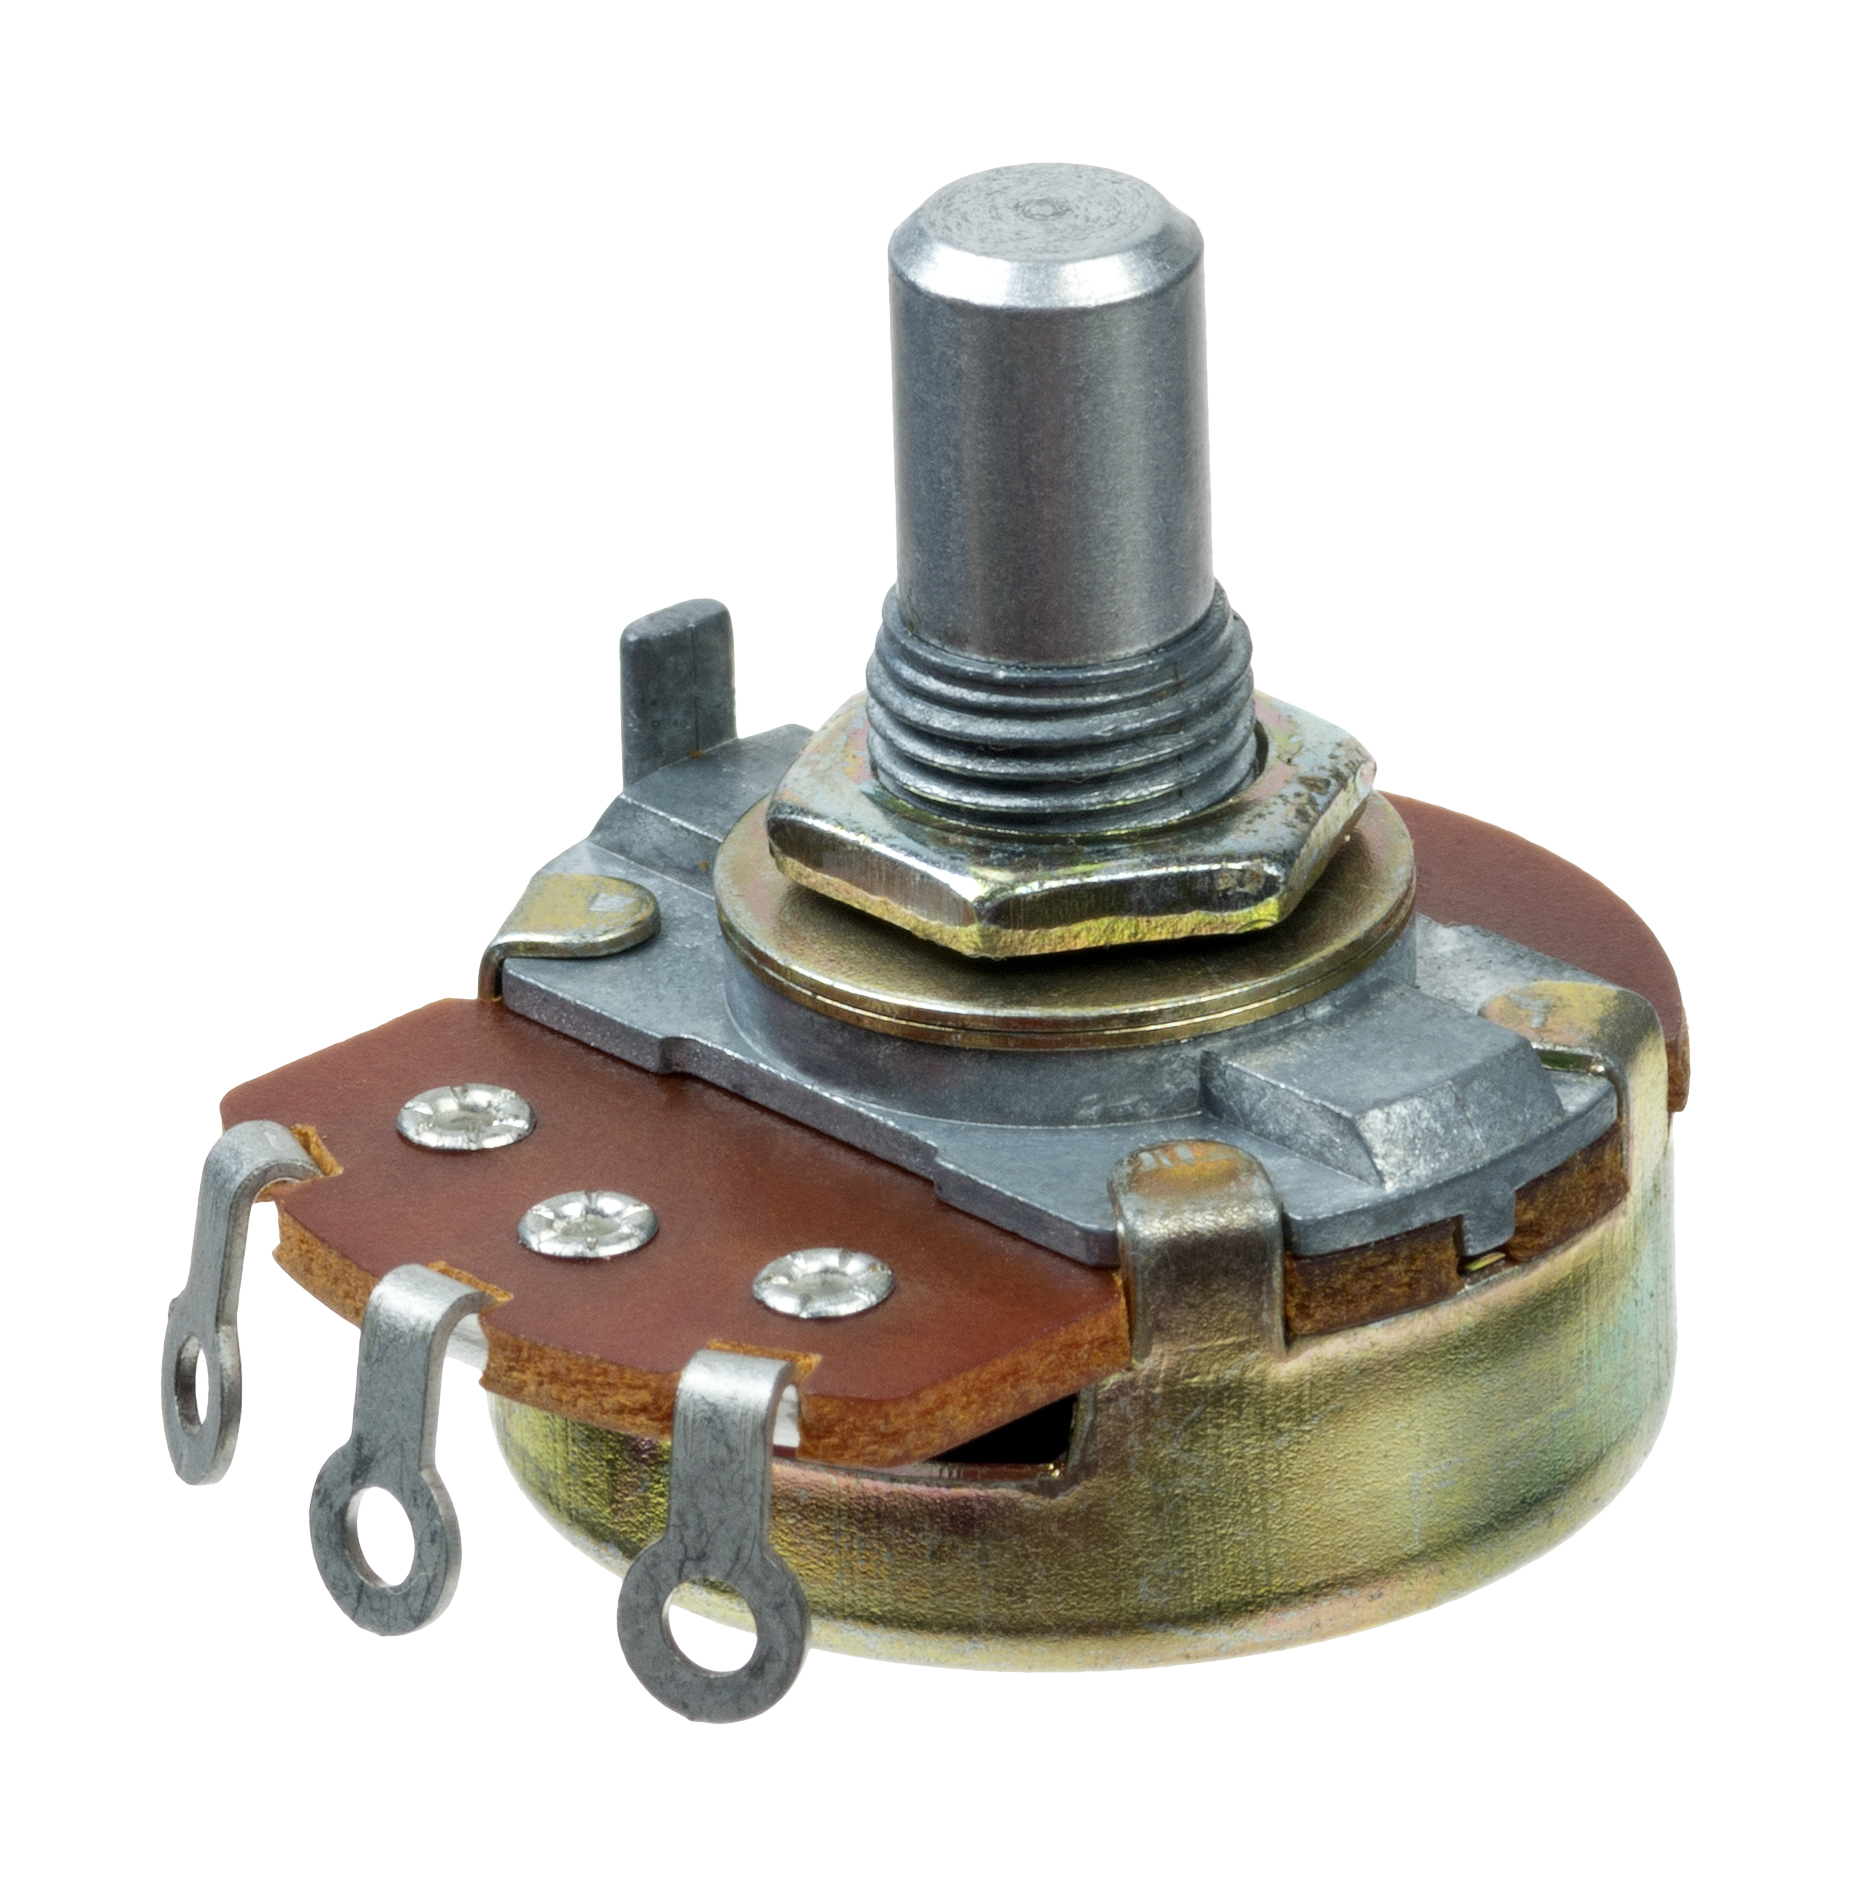
\includegraphics[width=0.95\textwidth, angle=0]{Meetings/February/02-17-22/02-17-22 1.jpg}
\caption{An example of a potentiometer}
\label{fig:021722_1}
\end{figure}

\begin{figure}[htp]
\centering
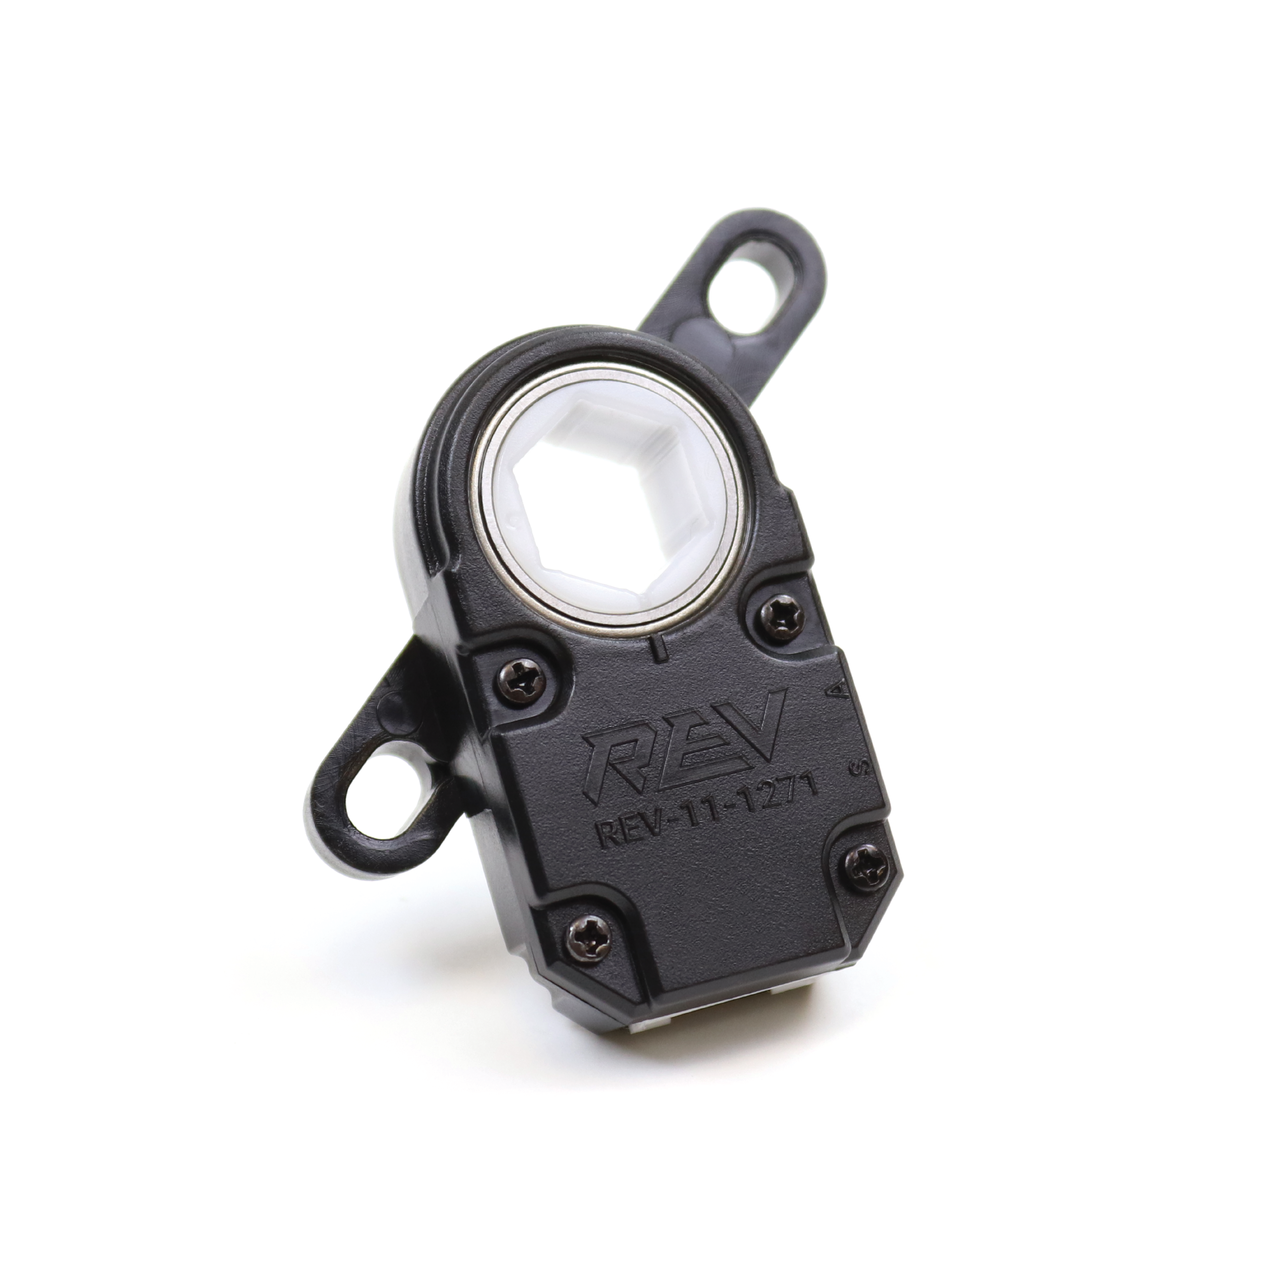
\includegraphics[width=0.95\textwidth, angle=0]{Meetings/February/02-17-22/02-17-22 2.PNG}
\caption{REV Through Bore encoder}
\label{fig:021722_2}
\end{figure}

\hhscommittee{Hardware}
\noindent\hfil\rule{\textwidth}{.4pt}\hfil
\subsubsection*{Goals}
\begin{itemize}
    \item Use 3d printed jig to drill motor and bearing block holes
	\item Screw motor in and ensure they line up correctly


\end{itemize} 

\noindent\hfil\rule{\textwidth}{.4pt}\hfil

\subsubsection*{Accomplishments}
After getting the 3D printed jigs we made to line up the motor and bearing block holders, we immediately go to work setting them up. Because it is integral that they are aligned correctly relative to each other, we used a strip of wood and glued the two sides of the jig together (Figure \ref{fig:021722_3}). We used these to drill the holes then screwed the motor and bearing block onto the carbon fiber sides. Hoping that we had lined everything up properly, we pushed a shaft through the bearing block to check if it was at the right place to easily fit into the core hex motor screwed onto the other side. Much to our disappointment, we found that the shaft was a bit off. Although it was very close, we had a difficult time pushing the shaft into the motor because we hat to press it into the motor at an angle. Unsatisfied with this error, we widened the holes for the bearing block  from 3 mm to about 5.5 mm then used washers to screw the bearing block in tightly enough to hold it at a new height. This works because our margin of error was less than a millimeter off, so widening the holes so we can slide the bearing block up moves it just high enough to fit correctly with the motor (Figure \ref{fig:021722_4}). 



\begin{figure}[htp]
\centering
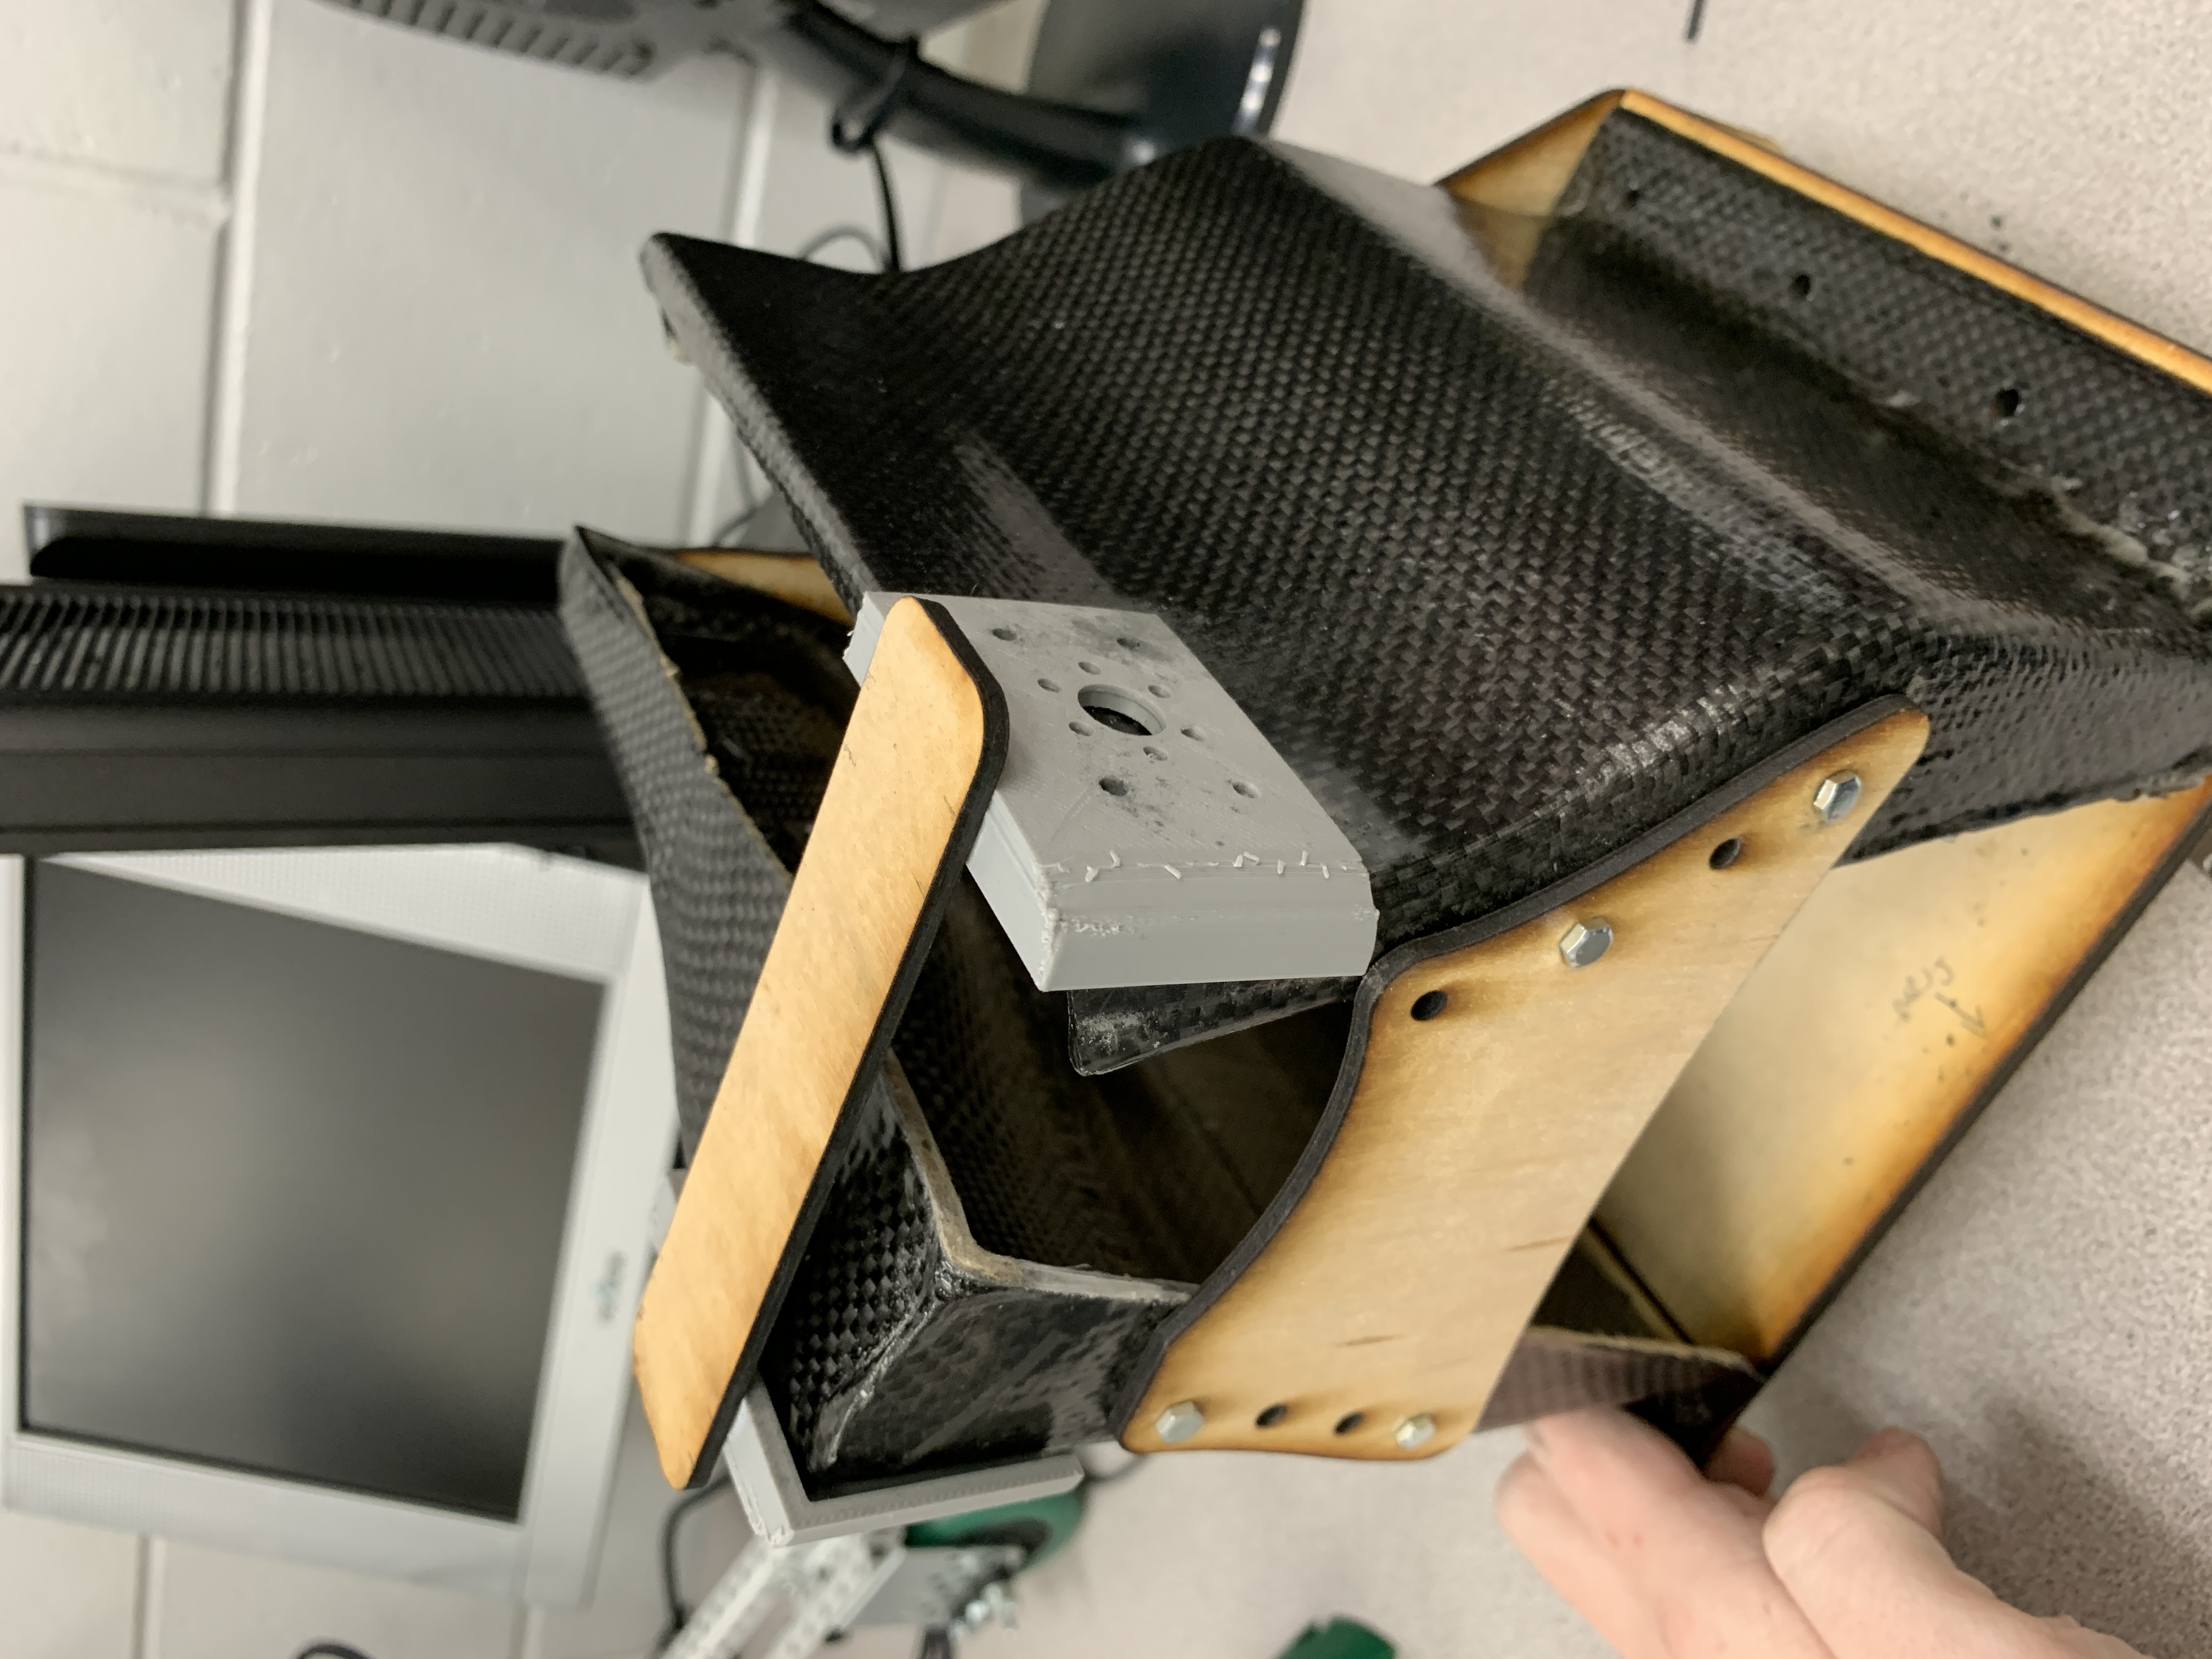
\includegraphics[width=0.95\textwidth, angle=0]{Meetings/February/02-17-22/2-17-22_Hardware_Figure1 - Nathan Forrer.JPG}
\caption{Glued together jig}
\label{fig:021722_3}
\end{figure}

\begin{figure}[htp]
\centering
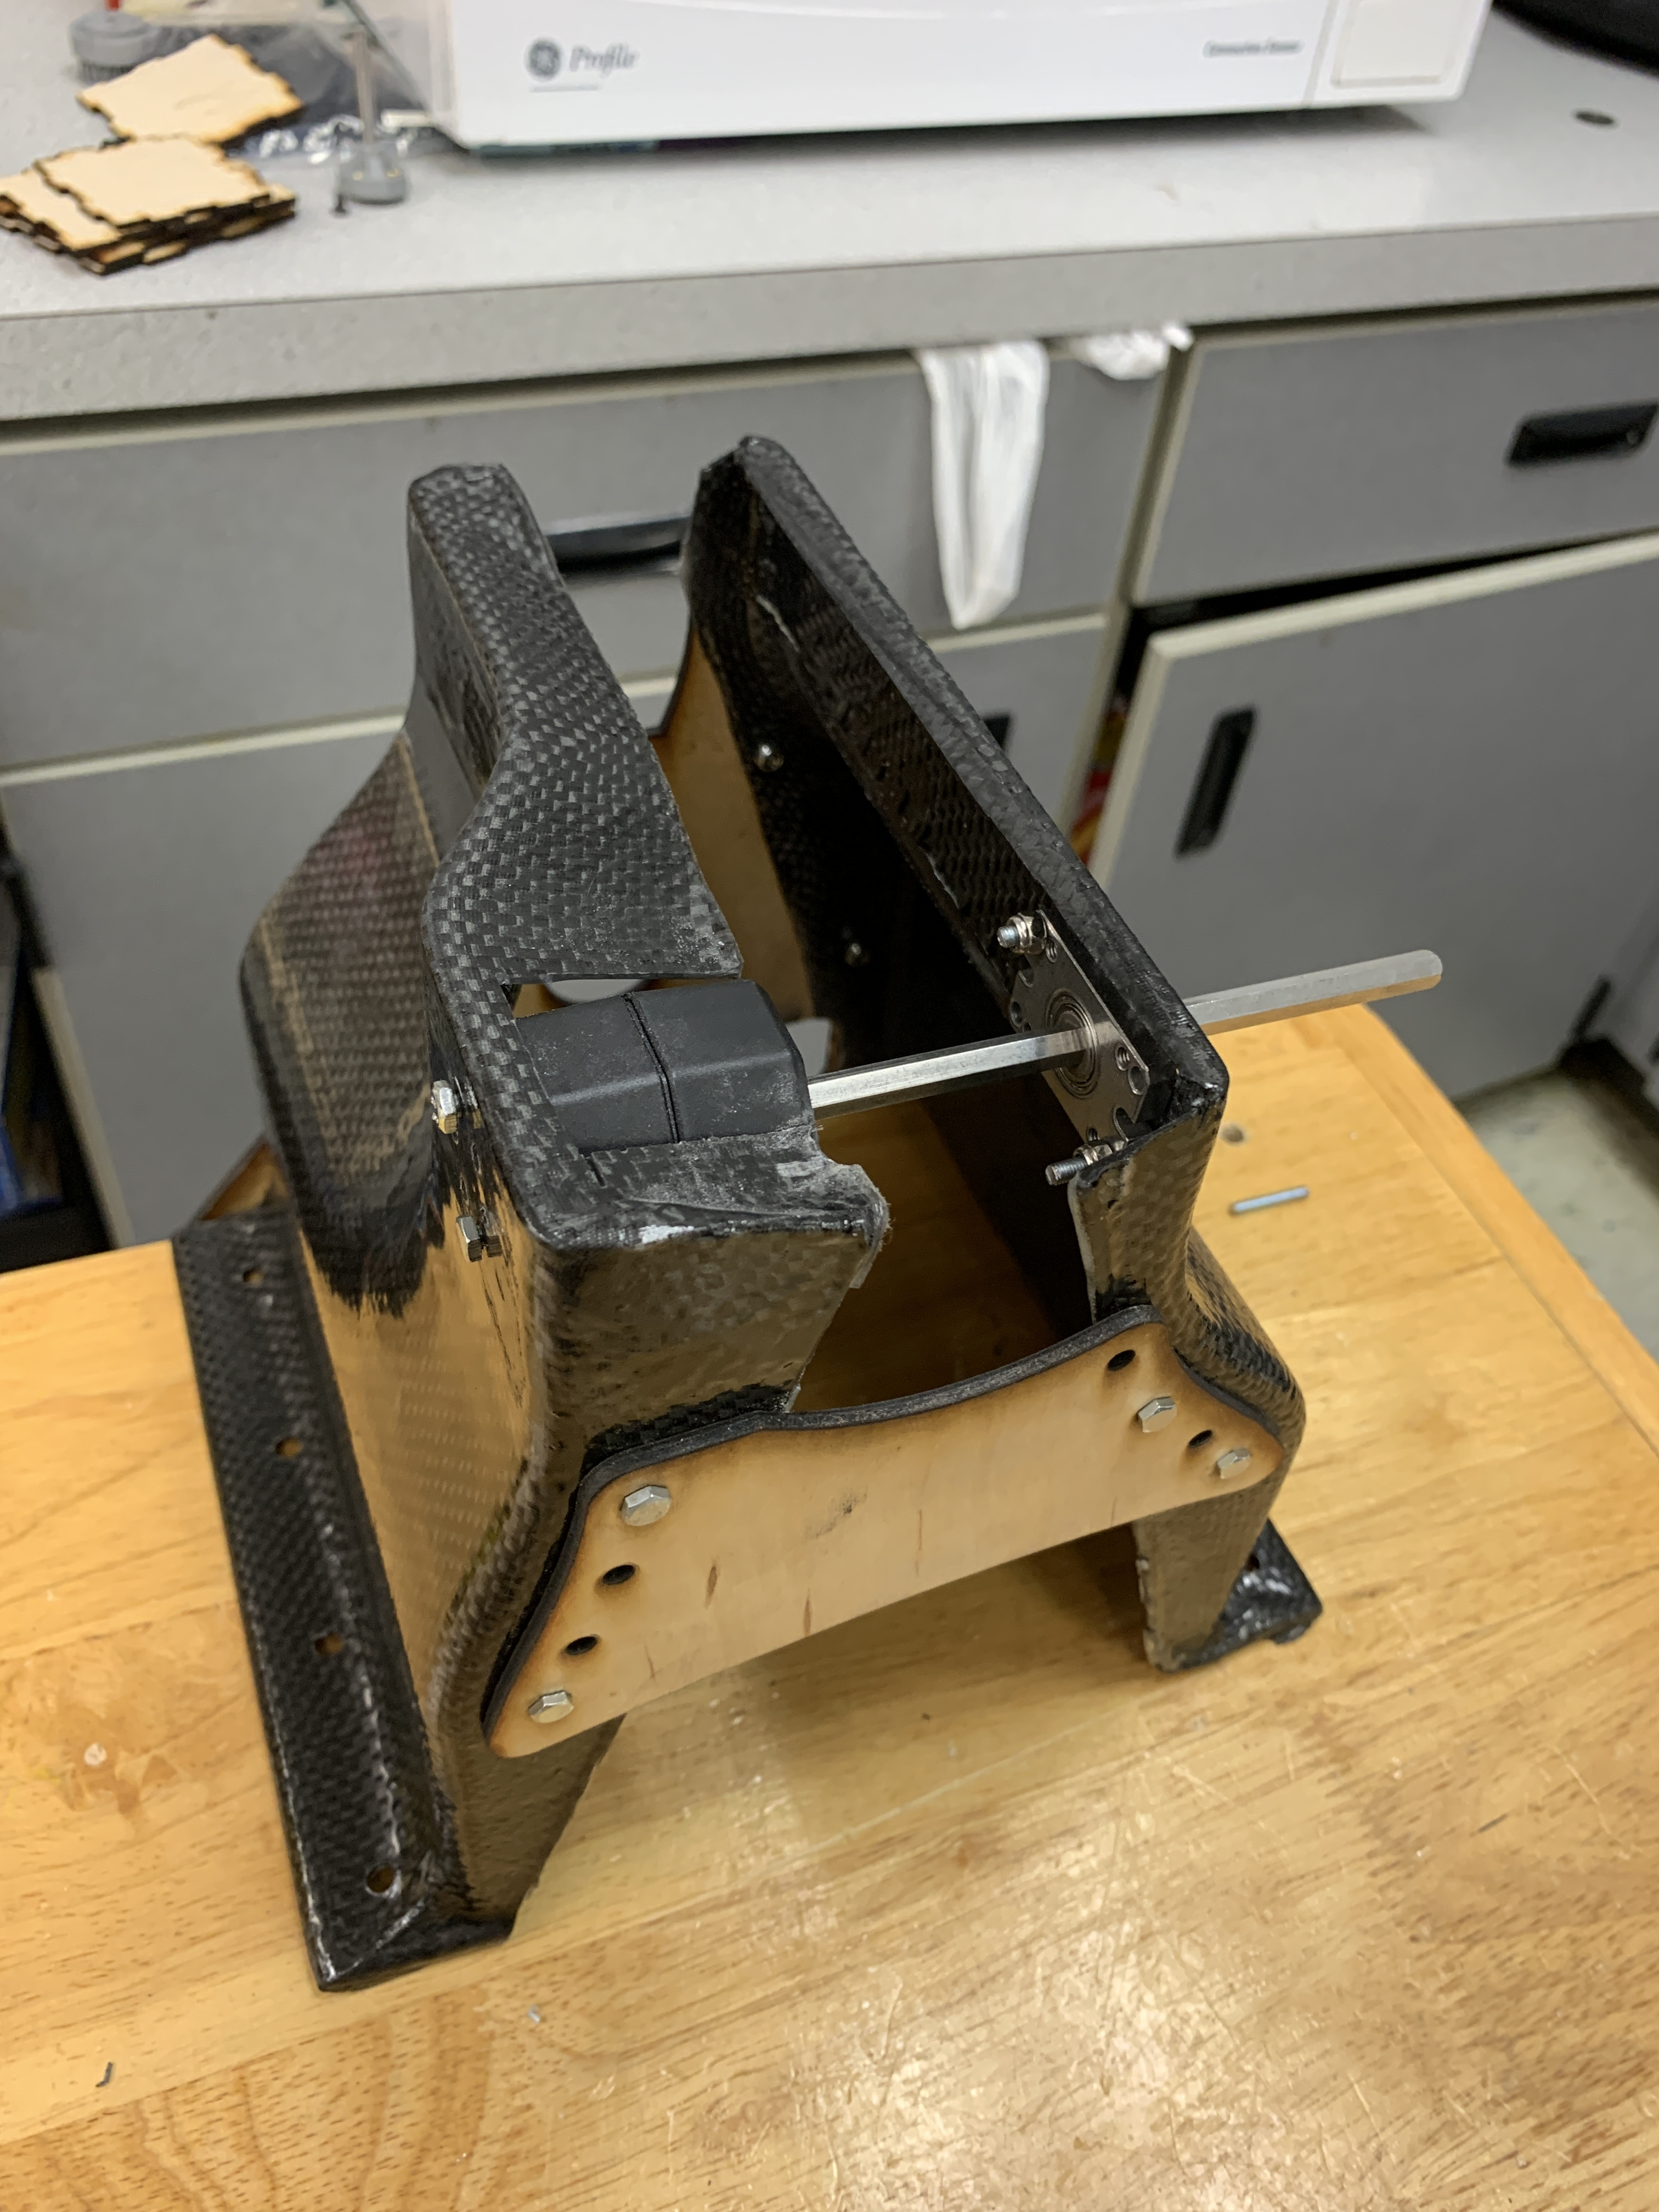
\includegraphics[width=0.95\textwidth, angle=0]{Meetings/February/02-17-22/2-17-22_Hardware_Figure2 - Nathan Forrer.JPG}
\caption{Bearing block}
\label{fig:021722_4}
\end{figure}


\whatsnext{
\begin{itemize}
    \item Improve our autonomous scoring consistency before the State competition. 
    \item rev extrusion arm supports
	\item Add carbon fiber arm supports 
	\item Wire manage

\end{itemize} 
}

